%  LaTeX support: latex@mdpi.com 
%  For support, please attach all files needed for compiling as well as the log file, and specify your operating system, LaTeX version, and LaTeX editor.

%=================================================================
\documentclass[foods,article,submit,moreauthors]{Definitions/mdpi} 
%\documentclass[journal,article,submit,moreauthors,unicode]{Definitions/mdpi} % For some letters Palatino lacks
%\documentclass[preprints,article,submit,moreauthors]{Definitions/mdpi} 
%\documentclass[preprints,article,submit,moreauthors,unicode]{Definitions/mdpi} 
% For posting an early version of this manuscript as a preprint, you may use "preprints" as the journal. Changing "submit" to "accept" before posting will remove line numbers.

%--------------------
% Class Options:
%--------------------
%----------
% journal
%----------
% Choose between the following MDPI journals:
% accountaudit, acn, acoustics, actuators, addictions, addictprev, adhesives, adolescents, aee, aerobiology, aeronautics, aerospace, agriculture, agriengineering, agrochemicals, agronomy, ai, aiagents, aichem, aieng, aimater, aimed, aipa, air, aisens, aisoc, algorithms, allergies, alloys, amh, analog, analytica, analytics, anatomia, anesthres, animals, antibiotics, antibodies, antioxidants, applbiosci, appliedchem, appliedmath, appliedphys, applmech, applmicrobiol, applnano, applsci, aps, aquacj, archaeolstud, architecture, arm, arthropoda, asc, asd, asi, astronautics, astronomy, atmosphere, atoms, audiolres, automation, axioms, bacteria, batteries, bcrc, bdcc, beverages, bioactives, biochem, bioengineering, biologics, biology, biomass, biomechanics, biomed, biomedicines, biomedinformatics, biomimetics, biomolecules, biophysica, bioresourbioprod, biosensors, biosphere, biotech, birds, blockchains, bloods, blsf, brainsci, breath, buildings, cancers, carbon, cardio, cardiogenetics, cardiovascmed, catalysts, cells, ceramics, challenges, chemeco, chemengineering, chemistry, chemosensors, chemproc, children, chips, cimb, civileng, cleantechnol, climate, clinbioenerg, clinpract, clockssleep, cmd, cmtr, coasts, coatings, colloids, colorants, commodities, complexities, complications, compounds, computation, computers, condensedmatter, conservation, constrmater, cosmetics, covid, crops, cryo, cryptography, crystals, csmf, ctn, culture, curroncol, cyber, dairy, data, ddc, dentistry, dermato, dermatopathology, designs, devices, dgg, dhi, diabetology, diagnostics, dietetics, digital, disabilities, diseases, diversity, dna, drones, drugreact, drylands, dynamics, earth, ebj, ece, ecm, ecologies, edm, eesp, electricity, electrochem, electronicmat, electronics, embodiedintell, encyclopedia, endocrines, energies, eng, engproc, entomology, entropy, environments, environremediat, enzymology, epidemiologia, epigenomes, epilepsy, esa, est, fermentation, fibers, fintech, fire, fishes, fluids, foodeng, foods, forecasting, forensicsci, forests, fossstud, foundations, fractalfract, freshwater, fuels, future, futureinternet, futurepharmacol, futurephys, futuretransp, galaxies, gases, gastroent, gastrointestdisord, gastronomy, gels, genes, geochem, geographies, geohazards, geomatics, geometry, geosciences, geotechnics, geriatrics, germs, glacies, grainsci, grasses, green, greenhealth, gucdd, gynecolcancer, hardware, hazardousmatters, healthcare, healthcmater, hearts, hemato, hematolrep, hep, heritage, higheredu, highthroughput, horticulturae, hospitals, humanoids, hydrobiology, hydrogen, hydrology, hydrometeorology, hydropower, hygiene, idr, iic, ijem, ijerph, ijgi, ijmd, ijms, ijns, ijom, ijp, ijpb, ijt, ijtm, ijtpp, ijtst, ime, immuno, industries, inflammj, informatics, information, infrastructures, inorganics, insects, instruments, inventions, iot, iron, j, jaestheticmed, jal, japma, jcdd, jcm, jcp, jcrm, jcs, jcto, jdad, jdb, jdcp, jdream, jemr, jeta, jfb, jfmk, jfth, jgbg, jgg, jimaging, jlpea, jmahp, jmmp, jmms, jmp, jmse, jne, jnt, jof, joitmc, joma, jop, joptm, jor, jox, jpbi, jphytomed, jpm, jsan, jtaer, jvd, jzbg, kidneydial, kinasesphosphatases, knowledge, labmed, laboratories, lam, land, langtechnol, lasers, legumes, life, lights, limnolrev, lipidology, liquids, livers, logics, logistics, lubricants, lymphatics, machines, macromol, magnetism, magnetochemistry, make, marinedrugs, maritime, materials, materproc, mathematics, mca, mcb, measurements, meb, medicina, medicines, medsci, membranes, merits, metabolites, metals, metamaterialsadv, meteorology, methane, metrics, metrology, micro, microarrays, microbiolres, microelectronics, micromachines, microorganisms, microplastics, microwave, minerals, mining, mmphys, modelling, molbank, molecules, mollusca, mps, msf, mti, multimedia, muscles, mutation, nanoenergyadv, nanomanufacturing, nanomaterials, ncrna, ndt, network, neuroglia, neuroimaging, neurolint, neurosci, nitrogen, notspecified, nursrep, nutraceuticals, nutrients, obesities, occuphealth, oceans, ohbm, onco, optics, optoelectronics, oral, organics, organoids, osteology, oxygen, pandemics, parasites, parasitologia, particles, pathogens, pathophysiology, pediatrrep, pets, pharmaceuticals, pharmaceutics, pharmacoepidemiology, pharmacy, phc, philosophies, photochem, photonics, photovoltaics, phycology, physchem, physics, physiologia, plants, plasma, platforms, pnr, pollutants, polymers, polysaccharides, populations, poultry, powders, precision, precisoncol, preprints, prevhealthc, proceedings, processes, prosthesis, proteomes, psf, psychiatryint, psychoactives, purification, quantumrep, quaternary, qubs, radiation, rareearths, rdt, reactions, realestate, receptors, recycling, regeneration, remotesensing, reports, reprodmed, resources, rheumato, rjpm, robotics, rsee, ruminants, safety, sanpp, sca, sci, scipharm, sclerosis, seeds, sensors, senssyst, separations, sexes, shi, signals, sinusitis, siuj, skins, smartcities, smartfish, smartgrids, sna, societies, software, soilsystems, solar, solids, spectroscj, sports, standards, stats, std, stratsediment, stresses, strokerep, superintelligence, surfaces, surgeries, susagric, suschem, sustainability, sustainfoods, sustainpackag, symmetry, synbio, systems, tae, targets, taxonomy, technologies, telecom, test, textiles, thalassrep, therapeutics, thermo, timespace, tomography, toxics, toxins, tph, transplantology, transportation, traumacare, traumas, tri, tropicalmed, universe, urbansci, uro, vaccines, vehicles, venereology, vetsci, vibration, virtualworlds, viruses, vision, waste, water, welding, wem, wevj, wild, wind, women, world, zoonoticdis

%---------
% article
%---------
% The default type of manuscript is "article", but can be replaced by: 
% abstract, addendum, article, benchmark, book, bookreview, briefcommunication, briefreport, casereport, changes, clinicopathologicalchallenge, comment, commentary, communication, conceptpaper, conferenceproceedings, correction, conferencereport, creative, datadescriptor, discussion, entry, expressionofconcern, extendedabstract, editorial, essay, erratum, fieldguide, hypothesis, interestingimages, letter, meetingreport, monograph, newbookreceived, obituary, opinion, proceedingpaper, projectreport, reply, retraction, review, perspective, protocol, shortnote, studyprotocol, supfile, systematicreview, technicalnote, viewpoint, guidelines, registeredreport, tutorial, giantsinurology, urologyaroundtheworld, patentsummary

% supfile = supplementary materials

%----------
% submit
%----------
% The class option "submit" will be changed to "accept" by the Editorial Office when the paper is accepted. This will only make changes to the frontpage (e.g., the logo of the journal will get visible), the headings, and the copyright information. Also, line numbering will be removed. Journal info and pagination for accepted papers will also be assigned by the Editorial Office.

%------------------
% moreauthors
%------------------
% If there is only one author the class option oneauthor should be used. Otherwise use the class option moreauthors.

%=================================================================
% MDPI internal commands - do not modify
\firstpage{1} 
\makeatletter 
\setcounter{page}{\@firstpage} 
\makeatother
\pubvolume{1}
\issuenum{1}
\articlenumber{0}
\pubyear{2026}
\copyrightyear{2026}
%\externaleditor{Firstname Lastname} % More than 1 editor, please add `` and '' before the last editor name
\datereceived{ } 
\daterevised{ } % Comment out if no revised date
\dateaccepted{ } 
\datepublished{ } 
%\datecorrected{} % For corrected papers: "Corrected: XXX" date in the original paper.
%\dateretracted{} % For retracted papers: "Retracted: XXX" date in the original paper.
%\doinum{} % Used for some special journals, like molbank
%\pdfoutput=1 % Uncommented for upload to arXiv.org
%\CorrStatement{yes}  % For updates
%\longauthorlist{yes} % For many authors that exceed the left citation part
%\IsAssociation{yes} % For association journals


%=================================================================
% Add packages and commands here. The following packages are loaded in our class file: fontenc, inputenc, calc, indentfirst, fancyhdr, graphicx, epstopdf, lastpage, ifthen, float, amsmath, amssymb, lineno, setspace, enumitem, mathpazo, booktabs, titlesec, etoolbox, tabto, xcolor, colortbl, soul, multirow, microtype, tikz, totcount, changepage, attrib, upgreek, array, tabularx, pbox, ragged2e, tocloft, marginnote, marginfix, enotez, amsthm, natbib, hyperref, cleveref, scrextend, url, geometry, newfloat, caption, draftwatermark, seqsplit
\usepackage{longtable}
\usepackage{bm}

%=================================================================
% Full title of the paper (Capitalized)
\Title{Powtarzalność oceny typowości smaku i~zapachu miodu: ślepy panel konsumencki, a~werdykty czterech laboratoriów}

% Author Orchid ID: enter ID or remove command
\newcommand{\orcidauthorA}{0009-0004-1158-0693} % Bartosz Lewandowski
\newcommand{\orcidauthorB}{0000-0001-9178-1540} % Przemysław Rujna
\newcommand{\orcidauthorC}{0000-0003-2580-7954} % Katarzyna Joanna Banach
\newcommand{\orcidauthorD}{0000-0003-2580-7954} % Ewaryst Tkacz -- TODO: ORCID
\newcommand{\orcidauthorE}{0000-0003-3900-7368} % Anna Gajda
\newcommand{\orcidauthorF}{0000-0003-1865-2122} % Maciej Wróbel -- TODO: ORCID
\newcommand{\orcidauthorG}{0000-0002-6289-7234} % Radowslaw Dzik

% Authors, for the paper (add full first names)
\Author{Bartosz Lewandowski $^{1,}$*\orcidA{}, Przemysław Rujna $^{2}$\orcidB{}, Katarzyna Joanna Banach $^{3}$\orcidC{}, Ewaryst Tkacz $^{1}$\orcidD{}, Anna Gajda $^{4}$\orcidE{}, Radosław Dzik  $^{1}$\orcidG{} and Maciej Wróbel $^{5}$\orcidF{}}

% MDPI internal command: Authors, for metadata in PDF
\AuthorNames{Bartosz Lewandowski, Przemysław Rujna, Katarzyna Joanna Banach, Ewaryst Tkacz, Anna Gajda, Radosław Dzik,  Maciej Wróbel}

% TODO: zweryfikować afiliacje i adresy e-mail wszystkich autorów
\address{%
$^{1}$ \quad Department of Clinical Engineering, Academy of Silesia in Katowice, Poland\\
$^{2}$ \quad Wydział Nauk o Zarządzaniu, Uniwersytet Morski w Gdyni, Poland\\
$^{3}$ \quad Instytut Nauk o Zarządzaniu i Jakości, Uniwersytet Warmińsko-Mazurski w Olsztynie, Poland\\
$^{4}$ \quad Warsaw University of Life Sciences: Warsaw, Poland\\
$^{5}$ \quad Nicolaus Copernicus University Collegium Medicum: Bydgoszcz, Poland }

% Contact information of the corresponding author
\corres{Correspondence: bartosz.lewandowski@akademiaslaska.pl}

% Abstract (Do not insert blank lines, i.e. \\)
\abstract{
    Ocena organoleptyczna jest częścią oceny miodu, na podstawie której podejmuje się decyzję o~dopuszczeniu produktu do obrotu lub jego odrzuceniu, choć powtarzalność oceny smaku jest trudna do zweryfikowania. Przeprowadzone badanie miało na celu weryfikację zgodności ocen między laboratoriami oraz między laboratoriami a~konsumentami. Badanie obejmowało ocenę siedmiu partii miodu dwiema niezależnymi metodami: w~ślepym teście konsumenckim (138~respondentów, 966~ocen) oraz w~ocenie organoleptycznej zleconej równolegle czterem laboratoriom. Ranking próbek w~panelu konsumenckim był zbieżny z~rankingiem laboratoryjnym ($\rho = 0{,}87$), lecz zbieżność ta wynikała z~ocen próbek skrajnych: po wyłączeniu jedynej próbki jednoznacznie typowej panel nie różnicował pozostałych sześciu ($p = 0{,}274$), a~ocena typowości próbek jednogłośnie zakwestionowanych przez laboratoria nie różniła się istotnie od 0{,}5. Zgodność trzech laboratoriów oceniających, czy smak miodu jest typowy, była umiarkowana ($\kappa = 0{,}60$) na skali binarnej i~słaba ($\kappa = 0{,}33$) na skali trzystopniowej, natomiast czwarte laboratorium wskazało ,,cechy niejednoznaczne'' dla wszystkich próbek. Pojedyncza ocena konsumenta odtwarzała werdykt większości laboratoriów na poziomie AUC 0{,}57. Ocena typowości smaku dostarcza informacji opisowej i~pozwala zgodnie identyfikować próbki skrajne, lecz w~przypadku próbek granicznych jej powtarzalność jest ograniczona. Stosowana samodzielnie, bez uwzględnienia miary zgodności między oceniającymi, nie spełnia wymogów stawianych kryterium oceny jakości handlowej.
}
% \abstract{Ocena organoleptyczna jest częścią oceny miodu, na podstawie której podejmowana jest decyzja o dposzuczeniu lub odrzuceniu produktu na rynek, chociaz powtarzalność werdyktu ,,smak nietypowy'' rzadko jest weryfikowana. Siedem partii miodu oceniono dwiema niezależnymi drogami: w~ślepym teście konsumenckim (138~respondentów, 966~ocen) oraz w~ocenie organoleptycznej zleconej równolegle czterem laboratoriom. Ranking typowości w~panelu był zbieżny z~rankingiem laboratoryjnym ($\rho = 0{,}87$), lecz zbieżność wynikała z~próbek skrajnych: po wyłączeniu jedynej próbki jednoznacznie typowej panel nie różnicował pozostałych sześciu ($p = 0{,}274$), a~typowość próbek jednogłośnie zakwestionowanych przez laboratoria nie różniła się istotnie od 0{,}5. Zgodność trzech laboratoriów stosujących kwalifikator typowości była umiarkowana ($\kappa = 0{,}60$) na skali binarnej i~słaba ($\kappa = 0{,}33$) na trzystopniowej, a~czwarte laboratorium orzekło ,,cechy niejednoznaczne'' dla wszystkich próbek. Pojedyncza ocena konsumenta odtwarzała werdykt większości laboratoriów na poziomie AUC 0{,}57. Ocena typowości smaku niesie informację opisową i~zgodnie identyfikuje próbki skrajne, lecz dla próbek granicznych nie jest powtarzalna. Stosowana samodzielnie i~bez miary zgodności oceniających nie spełnia wymogów stawianych kryterium oceny jakości handlowej.}


% Keywords
\keyword{miód; ocena organoleptyczna; ślepy test; panel konsumencki; zgodność międzylaboratoryjna; typowość smaku; jakość handlowa}

%%%%%%%%%%%%%%%%%%%%%%%%%%%%%%%%%%%%%%%%%%
\begin{document}

\section{Wprowadzenie}

Miód jest produktem, którego jakość ocenia się nie tylko za pomocą analiz
instrumentalnych, lecz także zmysłami: wzrokiem, węchem i~smakiem. Ocena
organoleptyczna jest tania i~szybko wykonalna, a~jej wynik ma znaczenie
praktyczne, ponieważ może zdecydować o~dopuszczeniu partii do obrotu.
Jednocześnie jest ona najtrudniejsza do ujednolicenia, bo opiera się na
ocenie człowieka, a~nie na odczycie przyrządu. Ramy prawne tej oceny
wyznaczają przepisy unijne, krajowe oraz normy międzynarodowe.

Jakość handlowa miodu dopuszczonego do obrotu w~Unii Europejskiej jest
określona dyrektywą 2001/110/WE \cite{Dyrektywa2001110}. Dyrektywa jest
implementowana w~prawie krajów członkowskich, a~poza Unią punktem odniesienia
jest norma Codex Alimentarius CXS 12-1981 \cite{CodexHoney}. Oba dokumenty,
obok parametrów oznaczanych instrumentalnie, zawierają wymagania
organoleptyczne. Miód nie może mieć obcego smaku ani zapachu, a~nazwę
odmianową można stosować tylko wtedy, gdy produkt wykazuje cechy
organoleptyczne, fizykochemiczne i~mikroskopowe właściwe dla deklarowanego
źródła.

Przepisy polskie stawiają wymaganie szersze. Rozporządzenie w~sprawie
jakości handlowej miodu \cite{RozporzadzenieMRiRW2003} uznaje za zgodny miód,
który ,,nie posiada zapachu i~smaku nietypowego dla danej odmiany miodu''.
Smak obcy pochodzi spoza miodu, na przykład z~substancji wchłoniętych podczas
przetwarzania i~przechowywania. Stwierdzenie smaku nietypowego wymaga
natomiast porównania z~wzorcem odmiany, którego żaden z~wymienionych aktów
nie definiuje. Charakterystyki opisowe głównych europejskich miodów
odmianowych opracowano w~literaturze \cite{PersanoOddo2004}, a~metodykę ich
oceny sensorycznej w~ramach International Honey Commission
\cite{Piana2004}, lecz nie mają one statusu wzorca prawnego. Jednocześnie
art.~5 dyrektywy zakazuje państwom członkowskim przyjmowania przepisów
krajowych dotyczących miodu, których dyrektywa nie przewiduje.

Metodę oceny organoleptycznej określa w~Polsce rozporządzenie w~sprawie metod
analiz miodu \cite{RozporzadzenieMRiRW2009}. Ogranicza się ono do wskazania,
że barwę, konsystencję, smak i~zapach bada się narządami wzroku, węchu
i~smaku, a~wyniki zestawia w~tabeli. Nie określa liczby ani kwalifikacji
oceniających, materiału odniesienia ani kryterium uznania smaku za
nietypowy. Dyrektywa (UE) 2024/1438, stosowana od 14~czerwca 2026~r.
\cite{Dyrektywa20241438}, przewiduje przyjęcie zharmonizowanych metod
wykrywania zafałszowań miodu, lecz nie metody oceny organoleptycznej.

Sposób przeprowadzenia oceny i~interpretacji jej wyniku pozostaje więc
w~gestii laboratorium. W~rezultacie werdykt organoleptyczny może samodzielnie
przesądzać o~niezgodności partii, nawet gdy pozostałe oznaczenia nie budzą
zastrzeżeń.

Od kryterium o~skutkach prawno-administracyjnych oczekuje się
obiektywności, powtarzalności i~proporcjonalności. W~kontroli urzędowej
wymóg ten ma podstawę prawną: metody badań laboratoryjnych muszą być zgodne
z~przepisami Unii, a~w~ich braku z~protokołami uznanymi międzynarodowo,
z~przepisami krajowymi lub zwalidowane w~badaniach między- lub
wewnątrzlaboratoryjnych \cite[art.~34]{Rozporzadzenie2017625}.
W~skoordynowanym planie kontroli miodu Komisji Europejskiej z~2015~r. test
sensoryczny włączono do pierwszego etapu charakterystyki próbek, obok
przewodności elektrycznej, aktywności diastazy i~analizy pyłkowej, jako
badanie wskazujące kierunek dalszych, bardziej specyficznych oznaczeń
\cite{KE2015PlanKontroli}. Mierzalność cechy nie
przesądza jeszcze o~jej przydatności jako kryterium decyzyjnego: wykazano to
dla mikrobiologicznych parametrów miodu, gdzie sama liczba drożdży
osmofilnych, bez oznak aktywnej fermentacji, nie stanowi wystarczającej
podstawy do zakwestionowania produktu \cite{Gajda2026}. Analogiczne pytanie
można postawić wobec oceny typowości smaku i~zapachu.

Literatura psychofizyczna wskazuje na dwa niezależne źródła zmienności takiej
oceny. Pierwszym jest międzyosobnicza, częściowo dziedziczna zmienność
percepcji smaków podstawowych: próg rozpoznania kwaśności jest dziedziczny
w~około 53\% \cite{wise2007twin}, a~polimorfizmy genu \textit{GNAT3}
wyjaśniają około 13\% wariancji percepcji słodyczy sacharozy
\cite{fushan2010sweet}. Ta sama próbka wywołuje więc u~różnych osób wrażenia
o~realnie różnej intensywności, a~doświadczeń zmysłowych nie da się
bezpośrednio porównać \cite{bartoshuk2000comparing}. Drugim źródłem jest
nieporównywalność skal opisowych: etykiety słowne (np.\ ,,bardzo silny'',
,,typowy'') oznaczają dla różnych osób różne intensywności bezwzględne,
co czyni skale kategorialne niewłaściwym narzędziem porównań między osobami
i~grupami \cite{bartoshuk2003labeled}.

Celem badania było empiryczne sprawdzenie, czy ocena typowości smaku i~zapachu
miodu jest na tyle powtarzalna, by mogła stanowić samodzielne kryterium
oceny jakości handlowej.
W~tym celu porównano wyniki ślepego testu konsumenckiego z~ocenami 
organoleptycznymi tych samych próbek, przeprowadzonymi niezależnie 
przez laboratoria. Analiza koncentrowała się na zdolności panelu konsumenckiego do różnicowania próbek pod względem typowości smaku, zgodności ocen między laboratoriami oraz stopniu, w~jakim konsumenci i~laboratoria wskazywali te same próbki jako nietypowe.

\section{Materiał i~metody}

\subsection{Próbki miodu}
\label{sub:probki}

Badaniom poddano siedem partii miodu, oznaczonych symbolami P1--P7. 
Następnie te  siedem partii miodu oceniono organoleptycznie dwiema
niezależnymi metodami: (i)~w~ślepym panelu konsumenckim ($n = 138$
respondentów) (rozdz.~\ref{sub:dobor_panelu}) oraz (ii)~w~ocenie organoleptycznej zleconej równolegle
czterem laboratoriom (rozdz.~\ref{sub:interlab_metody}). Postawiono trzy pytania badawcze: (1)~czy ślepy panel konsumencki
różnicuje próbki pod względem typowości smaku; (2)~czy niezależne
laboratoria zgadzają się ze sobą co do typowości tych samych próbek; (3)~czy
panel i~laboratoria wskazują te same próbki jako nietypowe i~z~jaką siłą.



\subsection{Ślepy panel konsumencki}
\label{sub:dobor_panelu}

Panelistów rekrutowano losowo spośród osób spełniających trzy kryteria
włączenia: brak alergii lub nadwrażliwości na produkty pszczele, brak
czasowych lub stałych zaburzeń węchu i~smaku. Próbki zakodowano i~podawano
w~losowej kolejności, bez informacji o~odmianie, producencie
i~pochodzeniu. Zapewniono standaryzowane warunki oceny (temperatura podawania,
oświetlenie, neutralizacja podniebienia między próbkami). Każdy panelista
ocenił wszystkie siedem próbek.

Arkusz oceny, zbudowany z pytań jednokrotnego wyboru, obejmował dane panelisty (grupa wiekowa: $<$25, 25--45, 46--65,
$>$65 lat; płeć; częstotliwość spożywania miodu: codziennie lub kilka razy
w~tygodniu, raz w~miesiącu, okazyjnie) oraz dla każdej próbki:
(i)~ocena, czyli ogólna akceptowalność smaku na skali od~1 (nieakceptowalny) do~5
(bardzo mi odpowiada); (ii)~słodycz, (iii)~kwasowość i~(iv)~aromat (intensywność)
 na skali: za słaba / w~sam raz / za silna; (v)~typowość - ocenę, czy smak jest
typowy dla miodu naturalnego (tak / nie) (pytanie~(v) odpowiada kryterium
,,typowości'' stosowanemu w~ocenie laboratoryjnej i~stanowi główną zmienną
porównawczą). Arkusz zawierał również pole na dowolne uwagi panelisty.

\subsection{Ocena organoleptyczna w~laboratoriach}
\label{sub:interlab_metody} 

Po zakończeniu panelu te same siedem partii przekazano w~sierpniu 2026 roku
(10--17.08.2026) równolegle czterem laboratoriom: Quality Services
International GmbH (Brema), Eurofins Food Integrity Control Services GmbH
(Ritterhude), Intertek Food Services GmbH (Brema) oraz Instytutowi
Ogrodnictwa -- PIB, Zakładowi Pszczelnictwa w~Puławach, 
zakodowane w publikacji jako Lab1, Lab2, Lab3 oraz Lab4.
Laboratoria otrzymały próbki jako standardowe zlecenia komercyjne, bez kodowania
względem tożsamości handlowej i~bez wiedzy o~pozostałych zleceniach.
Ocenę organoleptyczną wykonano według metod własnych laboratoriów: ASU
L~00.90-6 (zmodyfikowana), ICS SOP 520-02, DIN~10964 (metoda akredytowana)
oraz PN-88/A-77626 \cite{PN8877626} w~połączeniu z~metodą określoną
w~rozporządzeniu w~sprawie metod analiz miodu \cite{RozporzadzenieMRiRW2009}
(metoda nieakredytowana). W~publikacji
wykorzystano wyłącznie wyniki oceny organoleptycznej (zapach i~smak).
Laboratoria opisano w~wynikach numerami 1--4; numeracja jest umowna.

Lab1, Lab2 oraz Lab3 opisywały zapach i~smak metodami opisowymi,
uzupełniając opis kwalifikatorem typowości. Żadne ze sprawozdań nie
definiowało tego kwalifikatora ani nie wskazywało wzorca odniesienia, a~jego
brzmienie wskazuje na dwa układy odniesienia. Określenie ,,typowy dla
miodu'' (\textit{honey-specific}, \textit{honigtypisch}) odnosi próbkę do
cech miodu naturalnego; ocenę przeciwną laboratoria wiązały z~niezgodnością
z~dyrektywą 2001/110/WE lub z~zaleceniem badania w~kierunku zafałszowania.
Określenie ,,typowy dla pożytku'' (\textit{source-specific},
\textit{trachttypisch}) odnosi próbkę do pożytku ustalonego w~analizie
pyłkowej i~stanowiło podstawę nazwy odmianowej; laboratorium 2 powoływało
w~tym zakresie niemieckie wytyczne dla miodu \cite{BMEL2011Honig}. W~ocenach pozytywnych
przeważało odniesienie do pożytku, w~negatywnych występowało wyłącznie
odniesienie do miodu. Opisy zakodowano regułowo na skali trzystopniowej, bez
rozróżniania układów odniesienia: T (typowy), L (lekko lub słabo typowy),
N (nietypowy dla miodu). Wynikiem laboratorium dla próbki była niższa z~ocen
zapachu i~smaku (jeżeli dla jednej z~cech nie podano kwalifikatora,
przyjmowano ocenę drugiej), a~ocenę N~traktowano jako zastrzeżenie
organoleptyczne. Lab4 porównywało cechy próbki z~wymaganiami dla polskich miodów odmianowych 
i~nie stosowało kwalifikatora typowości. Jego werdykt końcowy, ,,cechy niejednoznaczne'',
oznacza, że próbki nie można uznać jej za nietypową dla miodu, dlatego zakodowano go jako L. Wszystkie cztery
laboratoria uwzględniono na równi we wszystkich miarach. Kodowanie wykonano
automatycznie na podstawie dosłownych opisów ze sprawozdań
(Załącznik~\ref{app:interlab_raw}).

% ------------------------------------------------------------------------- %
%  PLIK GENEROWANY AUTOMATYCZNIE przez apka/app.py (render_latex).
%  Nie edytować out.tex ręcznie — zmiany wprowadzać w apka/template.latex.
% ------------------------------------------------------------------------- %

\subsection{Analiza statystyczna}
\label{sub:statystyka}

Analizy wykonano w~języku Python (\texttt{pandas}, \texttt{NumPy},
\texttt{SciPy}). Przyjęto poziom istotności $\alpha = 0{,}05$ i~testy
dwustronne. Ze względu na porządkowy charakter skal (1--3 i~1--5) oraz
binarny charakter typowości smaku stosowano metody nieparametryczne
i~metody dla danych jakościowych. Każdy respondent oceniał wszystkie siedem
próbek.

\textit{Ślepy panel.} Dla każdej próbki obliczono odsetek ocen ,,smak
typowy'' z~95\% przedziałem Wilsona \cite{Wilson1927} i~sprawdzono testem
dwumianowym, czy różni się on od 0{,}5 (brak przewagi żadnej z~odpowiedzi).
Zdolność panelu do różnicowania próbek oceniono testem $Q$ Cochrana dla
typowości \cite{Cochran1950} oraz testem Friedmana dla ogólnej akceptacji
-- dla wszystkich siedmiu próbek oraz po wyłączeniu próbki o~skrajnie
wysokiej typowości.

\textit{Laboratoria.} Zgodność między trzema laboratoriami stosującymi
kwalifikator typowości wyrażono współczynnikiem $\kappa$ Fleissa
\cite{Fleiss1971} (interpretacja wg \cite{LandisKoch1977}) dla skali
binarnej (zastrzeżenie / brak zastrzeżenia) i~trzystopniowej (N / L / T).

\textit{Panel a~laboratoria.} Zbieżność rankingu próbek w~panelu
i~w~laboratoriach oceniono korelacją rang Spearmana ($n = 7$ próbek).
Próbki jednogłośnie zakwestionowane przez laboratoria porównano z~próbkami
bez zastrzeżeń na poziomie respondenta: dla każdej osoby obliczono różnicę
średniej typowości (oraz ogólnej akceptacji) obu grup próbek i~poddano ją
testowi Wilcoxona dla par \cite{Wilcoxon1945}; wielkość efektu wyrażono jako
$d$~Cohena dla danych sparowanych \cite{Cohen1988}. Zdolność pojedynczej
oceny panelisty do odtworzenia werdyktu większości laboratoriów oceniono
polem pod krzywą ROC (AUC) \cite{HanleyMcNeil1982} oraz odsetkami błędów
reguły ,,próbka nietypowa, gdy panelista uznał smak za nietypowy''.

%,,, -- %
\section{Wyniki}

\subsection{Charakterystyka panelu}

W~badaniu wzięło udział \textbf{138}~respondentów, którzy
łącznie wystawili 966~ocen (po 7~na osobę). Według dat
w~arkuszu panelu próbki oceniano w okresie maj-lipiec 2026.
Panel tworzyło 71~kobiet (51{,}4\%) i~64~mężczyzn
(46{,}4\%); dla 3~osób nie podano płci.
Najliczniejszą grupę wiekową stanowiły osoby poniżej 25.~roku życia
($n = 51$; 37\%), następnie osoby w~wieku
25--45 lat ($n = 37$; 26{,}8\%) i~46--65 lat
($n = 36$; 26{,}1\%); powyżej 65.~roku życia było
13~osób (9{,}4\%), a~1~osoba nie podała
wieku. Miód codziennie lub kilka razy w~tygodniu spożywało
44~osób (31{,}9\%), raz w~miesiącu
35 (25{,}4\%), a~okazyjnie
55 (39{,}9\%); 4~osoby
nie udzieliły odpowiedzi.

\subsection{Profil organoleptyczny próbek w~ślepym panelu}

Profil organoleptyczny siedmiu próbek przedstawiono w~tabeli~\ref{tab:lots}.
Średnia ogólna akceptacja wyniosła 3{,}261 (SD~1{,}241),
a~odsetek ocen ,,smak typowy dla miodu naturalnego'' -- 0{,}563.
Wyraźnie wyróżniała się próbka~P3 (typowość 0{,}905); typowość
pozostałych sześciu próbek mieściła się w~wąskim przedziale od 0{,}438
(P6) do 0{,}558 (P1).

\begin{table}[H]
\caption{Profil organoleptyczny próbek w~ślepym panelu konsumenckim.
\emph{Ocena} -- średnia ogólna akceptacja (1--5); \emph{Typowość} -- odsetek
ocen ,,smak typowy dla miodu naturalnego''; \emph{Słodycz}, \emph{Kwasowość},
\emph{Aromat} -- średnia na skali 1--3 (1~=~za słaba, 2~=~w~sam raz,
3~=~za silna); $n$ -- liczba odpowiedzi na pytanie o~typowość.\label{tab:lots}}
\begin{adjustwidth}{-\extralength}{0cm}
\begin{tabularx}{\fulllength}{lcCCCCC}
\toprule
\textbf{Próbka} & $\boldsymbol{n}$ & \textbf{Ocena} &
\textbf{Typowość} & \textbf{Słodycz} & \textbf{Kwasowość} & \textbf{Aromat} \\
\midrule
P1 & 138 & 3{,}37 & 0{,}558 & 2{,}07 & 1{,}77 & 1{,}69 \\
P2 & 137 & 3{,}04 & 0{,}496 & 2{,}06 & 1{,}77 & 1{,}81 \\
P3 & 137 & 3{,}92 & 0{,}905 & 2{,}20 & 1{,}89 & 2{,}06 \\
P4 & 137 & 3{,}15 & 0{,}540 & 2{,}12 & 1{,}82 & 1{,}82 \\
P5 & 136 & 3{,}16 & 0{,}515 & 2{,}33 & 1{,}89 & 2{,}08 \\
P6 & 137 & 3{,}07 & 0{,}438 & 2{,}26 & 1{,}87 & 2{,}04 \\
P7 & 137 & 3{,}11 & 0{,}489 & 2{,}23 & 1{,}81 & 1{,}85 \\
\bottomrule
\end{tabularx}
\end{adjustwidth}
\end{table}

Panel istotnie różnicował próbki zarówno pod względem typowości
($n = 136$ respondentów z~kompletem odpowiedzi;
$Q = 94{,}00$, $df = 6$, $p < 0{,}001$), jak i~ogólnej
akceptacji ($n = 129$; Friedman $\chi^2 = 55{,}35$, $p < 0{,}001$). Po wyłączeniu
P3 różnice między pozostałymi sześcioma próbkami nie były istotne ani dla
typowości ($Q = 6{,}35$, $df = 5$, $p = 0{,}274$), ani dla
ogólnej akceptacji ($\chi^2 = 7{,}95$, $p = 0{,}159$). Tylko dla
1 z~7~próbek (P3) odsetek ocen ,,typowy'' różnił się istotnie
od 0{,}5 (tabela~\ref{tab:panel_lab}).

\subsection{Ocena organoleptyczna w~laboratoriach}

Zakodowane werdykty trzech laboratoriów stosujących kwalifikator typowości
zestawiono w~tabeli~\ref{tab:panel_lab}, a~pełne, dosłowne opisy
-- w~tabeli~\ref{tab:interlab_opisy} (Załącznik~\ref{app:interlab_raw}).
Wszystkie trzy laboratoria uznały zapach lub smak próbek P6, P7 za
nietypowy dla miodu, żadne nie zgłosiło zastrzeżeń do próbek P3, P4, P5,
a~próbki P1 i~P2 zakwestionowało tylko jedno laboratorium. Pełną zgodność
na skali binarnej uzyskano dla 5 z~7~próbek
($\kappa = 0{,}60$, zgodność umiarkowana), a~na skali trzystopniowej
tylko dla 3 z~7~próbek ($\kappa = 0{,}33$,
zgodność słaba).

Czwarte laboratorium (metoda PN-88/A-77626) nie posługiwało się
kwalifikatorem typowości i~dla wszystkich siedmiu próbek orzekło ,,cechy
niejednoznaczne''. W~opisach wskazało zapach charakterystyczny dla oznak
fermentacji w~P1, P5 i~P6, zapach nienaturalny w~P2 i~landrynkowy w~P7
(tabela~\ref{tab:interlab_opisy}). Próbka~P5 nie budziła przy tym
zastrzeżeń żadnego z~trzech pozostałych laboratoriów, a~P1 -- dwóch z~nich.

\subsection{Zestawienie panelu z~wynikami laboratoriów}

\begin{table}[H]
\caption{Ślepy panel konsumencki a~ocena organoleptyczna trzech laboratoriów.
$n$ -- liczba odpowiedzi w~panelu; \emph{Typowość} -- odsetek ocen
,,smak typowy'' z~95\% przedziałem Wilsona; $p$ -- test dwumianowy względem 0{,}5.
Kody laboratoriów: T -- typowy, L -- lekko lub słabo typowy, N -- nietypowy
dla miodu (niższa z~ocen zapachu i~smaku). \emph{Zastrz.} -- liczba
laboratoriów z~oceną N.\label{tab:panel_lab}}
\begin{adjustwidth}{-\extralength}{0cm}
\begin{tabularx}{\fulllength}{lcCCCcccc}
\toprule
 & \multicolumn{4}{c}{\textbf{Ślepy panel}} &
\multicolumn{4}{c}{\textbf{Laboratoria}} \\
\cmidrule(lr){2-5}\cmidrule(lr){6-9}
\textbf{Próbka} & $\boldsymbol{n}$ & \textbf{Typowość} & \textbf{95\% CI} &
$\boldsymbol{p}$ & \textbf{1} & \textbf{2} & \textbf{3} & \textbf{Zastrz.} \\
\midrule
P1 & 138 & 0{,}558 & 0{,}47--0{,}64 & 0{,}201 & N & L & T & 1/3 \\
P2 & 137 & 0{,}496 & 0{,}41--0{,}58 & 1{,}000 & N & L & L & 1/3 \\
P3 & 137 & 0{,}905 & 0{,}84--0{,}94 & $<$0{,}001 & T & L & T & 0/3 \\
P4 & 137 & 0{,}540 & 0{,}46--0{,}62 & 0{,}393 & L & L & L & 0/3 \\
P5 & 136 & 0{,}515 & 0{,}43--0{,}60 & 0{,}797 & L & L & T & 0/3 \\
P6 & 137 & 0{,}438 & 0{,}36--0{,}52 & 0{,}171 & N & N & N & 3/3 \\
P7 & 137 & 0{,}489 & 0{,}41--0{,}57 & 0{,}864 & N & N & N & 3/3 \\
\bottomrule
\end{tabularx}
\end{adjustwidth}
\end{table}

Ranking próbek w~panelu był zbieżny z~rankingiem laboratoryjnym
(tabela~\ref{tab:panel_lab}, rysunek~\ref{fig:panel_lab}): korelacja
Spearmana między typowością w~panelu a~średnim kodem laboratoriów wyniosła
$\rho = 0{,}87$ ($p = 0{,}010$; dla ogólnej akceptacji
$\rho = 0{,}82$, $p = 0{,}024$). Po wyłączeniu
próbki~P3 korelacja przestała być istotna ($\rho = 0{,}79$,
$p = 0{,}059$). Większościowa odpowiedź panelu (typowość
$< 0{,}5$) pokryła się z~większościowym werdyktem laboratoriów dla
6 z~7~próbek.

\begin{figure}[H]
\begin{adjustwidth}{-\extralength}{0cm}
\centering
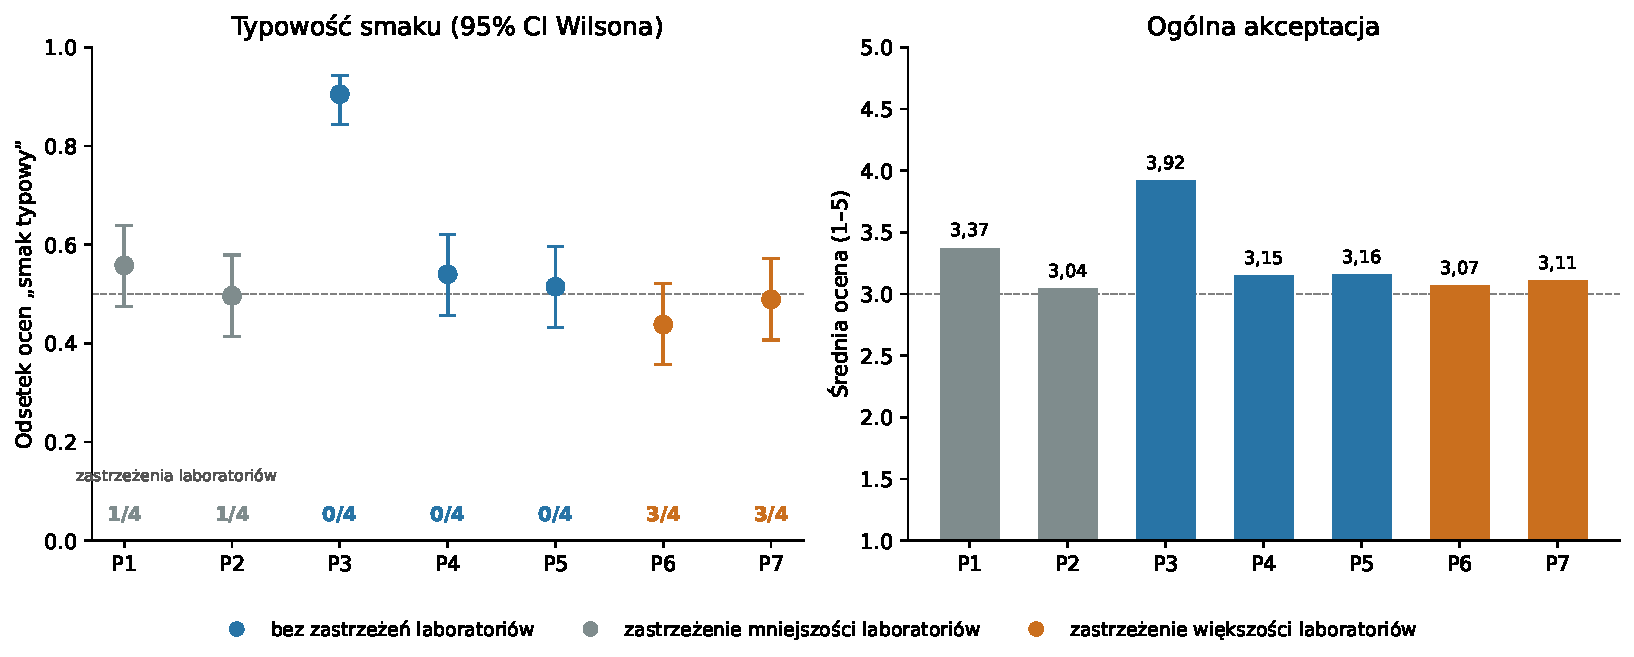
\includegraphics[width=16cm]{fig_panel_lab.pdf}
\end{adjustwidth}
\caption{Typowość smaku (punkty, 95\% przedział Wilsona) i~ogólna akceptacja
(słupki) siedmiu próbek w~ślepym panelu. Kolor oznacza werdykt laboratoriów:
niebieski -- brak zastrzeżeń, szary -- zastrzeżenie jednego laboratorium,
pomarańczowy -- zastrzeżenie wszystkich trzech; liczby u~dołu lewego panelu
-- liczba laboratoriów (z~trzech), które uznały zapach lub smak za nietypowy.
Linie przerywane -- 0{,}5 i~3.\label{fig:panel_lab}}
\end{figure}

Próbki jednogłośnie zakwestionowane przez laboratoria (P6, P7) uzyskały
w~panelu typowość 0{,}438 i~0{,}489 -- niższą od średniej, ale
nieodróżnialną od 0{,}5 ($p = 0{,}171$ i~$p = 0{,}864$). W~analizie
sparowanej typowość próbek bez zastrzeżeń laboratoryjnych (P3, P4, P5:
0{,}654) była wyższa niż próbek zakwestionowanych (P6, P7:
0{,}464); różnica wyniosła $\Delta = 0{,}189$ (95\% CI:
0{,}118--0{,}260; $p < 0{,}001$;
$d = 0{,}45$), a~dla ogólnej akceptacji $\Delta = 0{,}33$
punktu ($p = 0{,}002$) (rysunek~\ref{fig:contrast}). Po
wyłączeniu P3 różnica typowości spadła do $\Delta = 0{,}062$
i~przestała być istotna ($p = 0{,}144$).

\begin{figure}[H]
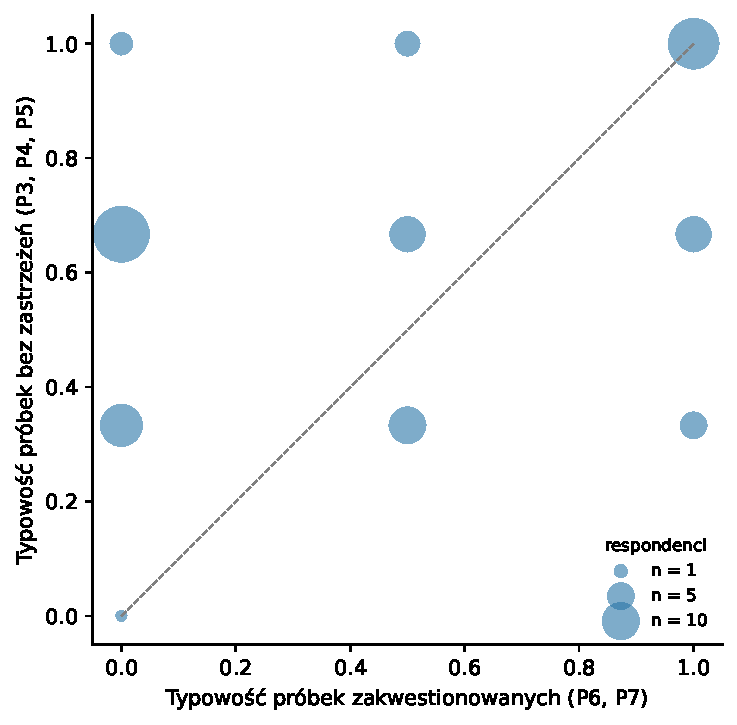
\includegraphics[width=8cm]{fig_contrast_lab.pdf}
\caption{Średnia typowość smaku próbek bez zastrzeżeń laboratoriów (oś~$y$)
i~próbek jednogłośnie zakwestionowanych (oś~$x$) dla każdego respondenta;
wielkość punktu -- liczba respondentów. Linia przerywana -- równość obu
ocen ($y = x$).\label{fig:contrast}}
\end{figure}

Pojedyncza ocena panelisty słabo odtwarzała werdykt większości laboratoriów
($\mathrm{AUC} = 0{,}570$, przy 0{,}5 dla zgadywania i~zwykle przyjmowanym
minimum 0{,}7 dla akceptowalnej dyskryminacji \cite{Hosmer2013}). Reguła ,,próbka nietypowa,
gdy panelista uznał smak za nietypowy'' wskazywałaby jako nietypowe
39{,}7\% ocen próbek, do których laboratoria nie miały zastrzeżeń,
i~uznawała za typowe 46{,}4\% ocen próbek przez nie
zakwestionowanych.

Panel zarejestrował natomiast cechę zbieżną z~częścią opisów
laboratoryjnych: słodycz oceniano jako ,,za silną'' najczęściej dla P5
(41{,}3\%), P6 (40{,}9\%) i~P7 (38{,}7\%), a~najrzadziej
dla P1 (22{,}1\%), P3 (22{,}6\%) i~P2 (24{,}1\%).
Czwarte laboratorium opisało jako ,,bardzo słodki'' smak P7, co zgadza się
z~oceną panelu, ale także smak P2, który panel rzadko oceniał jako zbyt
słodki.
 

Ślepy panel konsumencki i~laboratoria uporządkowały próbki podobnie pod względem
typowości, lecz nie były zgodne co do tego, które z~nich należy uznać za
nietypowe. Ranking typowości w~ślepym panelu konsumenckim
pokrywa się z~rankingiem laboratoryjnym: próbka~P3, bez zastrzeżeń
laboratoriów i~z~najwyższymi kodami laboratoryjnymi, była przez
konsumentów oceniana zdecydowanie najwyżej, a~próbki P6 i~P7, zakwestionowane
przez trzy z~czterech laboratoriów, znalazły się w~dolnej części
rankingu. Ocena smaku nie jest więc pozbawiona treści, ponieważ
odzwierciedla rzeczywiste różnice między miodami.

Zgodność ta wynikała jednak z~jednej próbki (P3), jedynej uznanej przez
ślepy panel konsumencki za typową. Po jej wyłączeniu panel nie różnicował pozostałych sześciu próbek ani pod względem typowości,
ani ogólnej akceptacji, a~typowość P6 i~P7 nie różniła się istotnie
od 0{,}5: mniej więcej połowa konsumentów uznała smak próbek
zakwestionowanych przez większość laboratoriów za typowy. Różnica między
próbkami zakwestionowanymi a~pozostałymi była istotna tylko dzięki P3
i~zanikała po jej wyłączeniu. Porównanie na tej samej skali pokazuje to
bezpośrednio. Panel jako całość nie zakwestionował żadnej próbki, a~przy
zaobserwowanej typowości rozstrzygnięcie dla P6 wymagałoby około
250~respondentów. Pojedynczy konsument zgadzał się z~laboratorium
w~57{,}5\% par ($\kappa = 0{,}10$), czyli w~podobnym stopniu jak z~innym
konsumentem ($\kappa = 0{,}08$), podczas gdy dwa laboratoria zgadzały się
w~71{,}4\% par ($\kappa = 0{,}30$). Ocena typowości rozpoznaje
zatem miód wyraźnie typowy, ale nie wyznacza ostrej granicy między miodem
,,typowym'' a~,,nietypowym'' -- a~właśnie takiej granicy wymaga kryterium
zgodności z~wymaganiami jakości handlowej.


\section{Dyskusja}

Skutki niskiej jakości ocen organoleptycznych najlepiej opisano na przykładzie
win. W badaniach nad sędziami winiarskimi tylko około 10\% z nich
potrafiło powtórzyć własną ocenę tej samej, zaślepionej próbki wina
w obrębie jednej kategorii \cite{hodgson2008judge}. Co więcej, zdobycie
wysokiej nagrody na jednym konkursie nie pozwalało przewidzieć wyniku na
innym: oba wyniki były statystycznie niezależne \cite{hodgson2009concordance}. 
Ocenę organoleptyczną można skalibrować poprzez selekcję i~trening asesorów,
monitorowanie wskaźników jakości panelu (powtarzalności, odtwarzalności,
zgodności) oraz stosowanie wzorców odniesienia i~skal o~zewnętrznym
zakotwiczeniu \cite{sipos2021panel,bartoshuk2004valid}. Dla miodu metodykę
taką opracowano w~ramach International Honey Commission \cite{Piana2004},
a~we Włoszech od 1999~r. prowadzony jest krajowy rejestr ekspertów analizy
organoleptycznej miodu, do którego wpis wymaga ukończenia szkoleń i~zdania
egzaminu \cite{AlboMiele1999}. \textcolor{purple}{We Francji metodykę oceny
organoleptycznej miodów odmianowych rozwinął zespół M.~Gonneta (INRA,
obecnie INRAE), od którego prac wywodzi się współczesna analiza
organoleptyczna miodu \cite{Piana2004}. W~Niemczech zasady oceny
organoleptycznej miodu opracowało Niemieckie Towarzystwo Rolnicze (DLG):
jako jej cele wskazano m.in. charakterystykę miodów odmianowych łącznie
z~analizą pyłkową oraz wykrywanie skutków przegrzania i~długiego
przechowywania, a~schemat oceny przewiduje dla zapachu i~smaku m.in. wady
,,nietypowy dla miodu'', ,,obcy zapach'' i~,,fermentujący'' \cite{DLG2015}.
W~obu krajach ocena organoleptyczna uzupełnia badania laboratoryjne, a~nie
je zastępuje.} W~rutynowej ocenie
miodu wskaźniki te zwykle nie są jednak publikowane w~sprawozdaniach, a~laboratoria
nie dysponują wspólnym materiałem odniesienia. Porównywalność werdyktów
organoleptycznych między laboratoriami pozostaje więc założeniem, a~nie
wykazaną właściwością pomiaru.

Ten sam wzorzec widać między laboratoriami. Zgodność czterech laboratoriów
była słaba na skali binarnej i~nieznaczna na skali trzystopniowej
\cite{LandisKoch1977}, a~pełna zgodność dotyczyła wyłącznie próbek, do
których żadne laboratorium nie miało zastrzeżeń. Próbki P1 i~P2
zakwestionowało tylko jedno z~czterech laboratoriów, podczas gdy pozostałe
opisały je jako typowe, lekko typowe lub o~cechach niejednoznacznych.
Lab4, stosujące inną metodę, orzekło ,,cechy niejednoznaczne'' dla
wszystkich siedmiu próbek, także dla P6 i~P7, zakwestionowanych przez
pozostałe trzy laboratoria, i~opisało zapach charakterystyczny dla oznak
fermentacji w~trzech próbkach, w~tym w~P5, do której żadne z~pozostałych
laboratoriów nie miało zastrzeżeń. Werdykt
dla tej samej partii zależy więc nie tylko od losowej zmienności percepcji,
lecz także od przyjętej metody i~laboratorium.

Rozbieżności te nie dowodzą błędu żadnego konkretnego laboratorium ani wady
konkretnej partii. Dowodzą natomiast, że typowość zapachu i~smaku nie jest
w~praktyce komercyjnej kontroli jakości mierzona powtarzalnie między
laboratoriami -- zgodnie z~przewidywaniami literatury psychometrycznej
\cite{bartoshuk2003labeled,hodgson2009concordance,sipos2021panel}. Etykieta
,,nietypowy'' jest wynikiem porównania z~wewnętrznym, niejawnym wzorcem
oceniającego, a~ten różni się między osobami i~laboratoriami.

\subsection{Opis cechy a~jej waga decyzyjna}

Panel zarejestrował cechę obecną w~części opisów laboratoryjnych: słodycz
P6 i~P7 częściej niż innych próbek oceniano jako ,,za silną'', a~próbki te
uzyskały najniższą typowość. Zależność ta nie była jednak jednoznaczna.
Konsumenci przypisali taką samą intensywność słodyczy próbce~P5, do której
laboratoria stosujące kwalifikator typowości nie miały zastrzeżeń. Próbkę~P2,
opisaną przez jedno z~laboratoriów jako ,,bardzo słodka'', oceniali natomiast
jako zbyt słodką rzadko.

Wyniki te sugerują, że opis organoleptyczny może trafnie oddawać cechę
próbki, a~mimo to nie odróżniać miodu typowego od nietypowego. Można to
tłumaczyć tym, że o~typowości decyduje nie sama intensywność pojedynczej
cechy, lecz jej zgodność z~profilem danej odmiany. Wymaga to jednak
dalszych badań. Dlatego warto odróżnić \emph{trafny opis} od
\emph{rozstrzygającego kryterium}: cecha może być przydatna do
charakterystyki produktu, a~jednocześnie nieprzydatna jako samodzielna
przesłanka decyzji administracyjnej \cite{Gajda2026}.

\subsection{Konsekwencje dla kontroli jakości}

Z~punktu widzenia kontroli istotne jest nie to, czy ocena smaku zawiera
jakąkolwiek informację, lecz czy pozwala powtarzalnie odtworzyć werdykt.
Pojedyncza ocena panelisty odtwarzała werdykt większości laboratoriów na
poziomie $\mathrm{AUC} = 0{,}57$ (95\% CI: 0{,}54--0{,}60), a~reguła oparta
na typowości smaku myliłaby się w~blisko co drugiej ocenie. Zgodność
konsumenta z~laboratorium ($\kappa = 0{,}10$) nie różniła się od zgodności
dwóch konsumentów ($\kappa = 0{,}08$). Same laboratoria zgadzały się w~pełni
co do trzech z~siedmiu próbek na skali binarnej i~jednej na skali
trzystopniowej. Kryterium, którego wynik dla próbek granicznych zależy od
wyboru oceniającego lub laboratorium, nie spełnia warunku powtarzalności,
a~użyte samodzielnie -- warunku proporcjonalności.

Różnicę tę widać w~samych sprawozdaniach. Lab2 i~Lab4 opisywały
regułę podejmowania decyzji z~uwzględnieniem niepewności pomiaru
\cite[pkt~7.8.6]{ISO17025} w~odniesieniu do wartości granicznych parametrów
mierzalnych, a~Lab4 wskazało wprost parametry fizykochemiczne
i~analizę pyłkową. Dla oceny organoleptycznej żadne sprawozdanie nie
podawało niepewności ani reguły decyzyjnej. W~przypadku metod
instrumentalnych precyzję wyznacza się w~badaniach międzylaboratoryjnych,
a~na jej podstawie ustala różnice krytyczne stosowane przy ocenie zgodności
z~kryteriami czystości miodu \cite{Ulberth2024}. Dla werdyktu ,,smak
nietypowy'' analogiczne wielkości nie są znane.

Nie oznacza to, że ocena organoleptyczna jest bezużyteczna. Jest cennym
narzędziem badania preferencji, opisu i~doskonalenia produktu, a~także
sygnałem do dalszych badań, w~roli przewidzianej dla testu organoleptycznego
w~skoordynowanym planie kontroli Komisji Europejskiej
\cite{KE2015PlanKontroli}, gdy wynik jest skrajny i~zgodny między
niezależnymi oceniającymi -- jak dla P6 i~P7. Podobną zależność opisano dla
wyszkolonych ekspertów: w~próbach International Honey Commission wyniki
oceny zgodności z~profilem miodu odmianowego były ważne dla próbek wyraźnie
dobrych lub wadliwych, natomiast dla próbek o~cechach pośrednich rozrzut
ocen był największy, a~binarna klasyfikacja ,,tak/nie'' nie dawała ważnego
wyniku w~23\% przypadków nawet po połączeniu trzech paneli
\cite{Piana2004}. \textcolor{purple}{Wyniki wskazują, że przy próbkach
granicznych werdykt organoleptyczny nie powinien być potwierdzany kolejną
oceną organoleptyczną prowadzoną bez wzorca. Drugie laboratorium,
posługujące się własnymi deskryptorami, dostarcza kolejnego opisu, a~nie
rozstrzygnięcia: jedno może określić smak jako ,,bardzo słodki'', inne
zapach jako ,,landrynkowy'', i~bez zdefiniowanego wzorca deskryptorów
typowości żaden z~tych opisów nie przesądza o~nietypowości. Werdykt ,,smak
nietypowy'' powinien zatem zostać zweryfikowany wynikami miarodajnymi:
oznaczeniami fizykochemicznymi i~mikroskopowymi, a~przy podejrzeniu
zafałszowania metodami analitycznymi o~znanej precyzji \cite{Ulberth2024},
zanim stanie się podstawą decyzji o~wycofaniu produktu. Rola oceny
organoleptycznej w~kontroli jakości handlowej powinna ograniczać się do
wykrywania cech nietypowych określonych w~przepisach, takich jak obcy smak
lub zapach oraz oznaki fermentacji
\cite{Dyrektywa2001110,RozporzadzenieMRiRW2009}, a~nie obejmować orzekania
o~typowości, dla której wzorzec nie istnieje.}

\textcolor{purple}{Takie ograniczenie odpowiada konstrukcji prawa unijnego.
Dyrektywa 2001/110/WE formułuje wymagania organoleptyczne w~postaci
zakazów: miód, z~wyjątkiem miodu piekarskiego, nie może mieć obcego smaku
ani zapachu i~nie może wykazywać oznak fermentacji \cite{Dyrektywa2001110}.
Ocena wyglądu, zapachu, smaku, konsystencji, krystalizacji i~widocznych
oznak fermentacji pozwala więc wskazać możliwą niezgodność i~uzasadnić
skierowanie próbki do dalszych badań laboratoryjnych. W~tej roli,
wstępnej i~uzupełniającej, a~nie jako samodzielną metodę analityczną,
wykorzystano test organoleptyczny w~skoordynowanym planie kontroli
Komisji Europejskiej \cite{KE2015PlanKontroli}.}

\subsection{Ograniczenia badania}
\label{sub:ograniczenia}

Najważniejszym ograniczeniem jest mała liczba partii. Choć panel wystawił
966~ocen, porównania na poziomie próbek (korelacja panel--laboratoria,
zgodność werdyktów) opierają się na siedmiu jednostkach. Po drugie, panel tworzyli
konsumenci po krótkim szkoleniu, a~nie wyselekcjonowani asesorzy; oddaje
to perspektywę rynkową, lecz zwiększa rozrzut ocen. Pytanie panelu
o~typowość smaku nie jest też tożsame z~procedurami laboratoryjnymi, które
oceniają łącznie zapach i~smak według własnych wzorców. Po trzecie, ocenę
laboratoryjną przeprowadzono jako zlecenia komercyjne, a~nie jako formalny
test pierścieniowy: próbki nie były kodowane, laboratoria nie dysponowały
wspólnym materiałem odniesienia, a~kodowanie ich opisów na skali T/L/N,
w~tym przypisanie werdyktowi ,,cechy niejednoznaczne'' kodu L, jest
uproszczeniem dokonanym przez autorów. Po czwarte, panel (maj--lipiec 2026)
i~ocenę laboratoryjną (sierpień 2026) dzieliło od jednego do trzech miesięcy,
w~czasie których cechy zależne od przechowywania (krystalizacja, fermentacja) mogły
się zmienić. Wreszcie, badano tylko siedem partii, dlatego wyników nie należy
uogólniać na wszystkie miody.

\section{Wnioski}

Ocena typowości smaku i~zapachu miodu prowadzona tak jak w~tym
badaniu (przez ślepy panel konsumencki lub przez pojedyncze
laboratorium, bez wspólnego wzorca odniesienia i~bez raportowanej miary
zgodności oceniających) jest zbyt zróżnicowana, by mogła być
rozstrzygającym parametrem oceny jakości handlowej próbki.

Przemawiają za tym trzy niezależne ustalenia. Po pierwsze, zdolność
dyskryminacyjna oceny jest nieakceptowalnie niska: pojedyncza ocena
panelisty odtwarzała werdykt laboratoriów z~$\mathrm{AUC} = 0{,}57$, czyli
na poziomie niewiele lepszym od wyboru binarnie losowej wartości ($\mathrm{AUC} = 0{,}5$)
i~wyraźnie poniżej wartości 0{,}7, uznawanej za minimum akceptowalnej
dyskryminacji \cite{Hosmer2013}. W~praktyce reguła ,,smak nietypowy --
próbka odrzucona'' zakwestionowałaby 39{,}7\% ocen próbek, do których
większość laboratoriów nie miała zastrzeżeń, i~przepuściła 46{,}4\% ocen
próbek przez nią zakwestionowanych, myliłaby się więc w~blisko co drugiej
decyzji. Po drugie, poza jedną wyraźnie typową próbką panel nie różnicował
próbek, a~jako całość nie zakwestionował żadnej z~nich: typowość próbek
zakwestionowanych przez większość laboratoriów (0{,}438 i~0{,}489) była
nieodróżnialna od 0{,}5. Po trzecie, oceniający nie byli zgodni ani między
sobą, ani z~laboratoriami: zgodność czterech laboratoriów była słaba na
skali binarnej ($\kappa = 0{,}30$) i~nieznaczna na skali trzystopniowej
($\kappa = 0{,}13$), a~pojedynczy konsument zgadzał się z~laboratorium
w~podobnym stopniu jak z~innym konsumentem ($\kappa = 0{,}10$
i~$\kappa = 0{,}08$).

Decyzja o~uznaniu partii za zgodną lub o~jej wycofaniu, oparta wyłącznie na
takim wyniku, zależałaby w~większym stopniu od tego, kto i~gdzie ocenia, niż
od właściwości samej próbki. Badanie subiektywne nie powinno więc stanowić
podstawy binarnej oceny „dobry/zły''. Ocena organoleptyczna zachowuje wartość
jako narzędzie opisowe i~sygnał do dalszych badań, zwłaszcza gdy wynik jest
skrajny i~zgodny między niezależnymi oceniającymi. Nie powinna jednak
samodzielnie rozstrzygać o~zgodności miodu z~wymaganiami jakości handlowej.
\textcolor{purple}{Ocena organoleptyczna powinna ograniczać się do
wykrywania cech nietypowych określonych w~przepisach, takich jak obcy smak
lub zapach oraz oznaki fermentacji, a~nie orzekać o~typowości, dla której
nie ma wzorca. Werdykt ,,smak nietypowy'' powinien być każdorazowo
weryfikowany wynikami miarodajnymi, a~nie kolejną oceną organoleptyczną
prowadzoną bez wzorca deskryptorów.}
\textcolor{purple}{W~konsekwencji decyzja o~uznaniu miodu za niezgodny
z~wymaganiami wyłącznie na podstawie nieokreślonego wrażenia
organoleptycznego, np.\ ,,zbyt słodki'', ,,niedostatecznie aromatyczny''
lub ,,niedostatecznie typowy'', byłaby podatna na zakwestionowanie, jeżeli
takiego kryterium nie określa prawo Unii, przepisy krajowe, specyfikacja
produktu ani uznana lub zwalidowana metoda badań
\cite[art.~34]{Rozporzadzenie2017625}.}


\vspace{6pt}

%%%%%%%%%%%%%%%%%%%%%%%%%%%%%%%%%%%%%%%%%%
% TODO (wymagane przez MDPI): uzupełnić i odkomentować poniższe oświadczenia.
%\authorcontributions{Conceptualization, B.L.; methodology, B.L. and P.R.; ... All authors have read and agreed to the published version of the manuscript.}
%\funding{This research received no external funding.}
%\institutionalreview{...}
%\informedconsent{Informed consent was obtained from all subjects involved in the study.}
%\dataavailability{...}
%\conflictsofinterest{...}

% \abbreviations{Abbreviations}{%
% W~pracy użyto następujących skrótów:\\

% \noindent
% \begin{tabular}{@{}ll}
% AUC & pole pod krzywą ROC (\emph{area under the curve})\\
% CI & przedział ufności (\emph{confidence interval})\\
% GEE & uogólnione równania szacujące (\emph{generalized estimating equations})\\
% LMM & liniowy model mieszany (\emph{linear mixed model})\\
% OR & iloraz szans (\emph{odds ratio})\\
% ROC & krzywa charakterystyki operacyjnej odbiornika
% \end{tabular}
% }

%%%%%%%%%%%%%%%%%%%%%%%%%%%%%%%%%%%%%%%%%%
\appendixtitles{yes}
\appendixstart
\appendix
\section[\appendixname~\thesection]{Dosłowne opisy zapachu i~smaku z~laboratoriów}
\label{app:interlab_raw}

Tabela~\ref{tab:interlab_opisy} zestawia dosłowne (przetłumaczone z~języka
angielskiego i~niemieckiego) opisy zapachu i~smaku zgłoszone przez laboratoria
(sierpień 2026, rozdz.~\ref{sub:interlab_metody}), stanowiące podstawę
kodowania w~tabeli~\ref{tab:panel_lab}.

% Dosłowne opisy z arkusza wyniki/Analiza_porownawcza_ODER_23_2026.xlsx
% (numeracja laboratoriów: 1 -- QSI, 2 -- Eurofins, 3 -- Intertek, 4 -- Puławy)
{\small
\begin{longtable}{@{}lc>{\raggedright\arraybackslash}p{5.2cm}>{\raggedright\arraybackslash}p{5.6cm}@{}}
\caption{Dosłowne opisy zapachu i~smaku zgłoszone przez cztery laboratoria
dla tych samych partii miodu (sierpień 2026). Numeracja
laboratoriów (1--4) jest umowna i~zgodna z~tabelą~\ref{tab:panel_lab}.\label{tab:interlab_opisy}}\\
\toprule
\textbf{Próbka} & \textbf{Lab.} & \textbf{Zapach} & \textbf{Smak} \\
\midrule
\endfirsthead
\multicolumn{4}{c}{\tablename\ \thetable{} (cd.)}\\
\toprule
\textbf{Próbka} & \textbf{Lab.} & \textbf{Zapach} & \textbf{Smak} \\
\midrule
\endhead
\bottomrule
\endfoot
P1
 & 1 & nietypowy dla miodu & nietypowy dla miodu \\
 & 2 & przypominający mocz zwierzęcy, lekko typowy dla pożytku & słodki, kwiatowy, łagodny, lekko typowy dla pożytku \\
 & 3 & typowy dla miodu & słodki, owocowy \\
 & 4 & słaby, lekko kwaśny, charakterystyczny dla oznak fermentacji & słodki, łagodny \\
\midrule
P2
 & 1 & nietypowy dla miodu & nietypowy dla miodu \\
 & 2 & przypominający mocz zwierzęcy, lekko typowy dla pożytku & słodki, kwiatowy, łagodny, lekko metaliczny, lekko typowy dla pożytku \\
 & 3 & lekko typowy dla pożytku & słodki, owocowy, lekko typowy dla pożytku \\
 & 4 & nienaturalny, lekko kwiatowy & bardzo słodki, szczypiący \\
\midrule
P3
 & 1 & typowy dla pożytku & typowy dla pożytku \\
 & 2 & lekko typowy dla pożytku & słodki, kwiatowy, ziołowy, lekko typowy dla pożytku \\
 & 3 & typowy dla miodu & słodki, kwiatowy, owocowy, ziołowy \\
 & 4 & silny, podobny do wosku pszczelego & słodki, nieco ostry \\
\midrule
P4
 & 1 & słabo typowy dla pożytku & słabo typowy dla pożytku \\
 & 2 & lekko typowy dla miodu & słodki, owocowy, medyczny (apteczny), lekko metaliczny, lekko typowy dla miodu \\
 & 3 & lekko typowy dla pożytku & słodki, owocowy, miętowy, lekko typowy dla pożytku \\
 & 4 & słabo wyczuwalny, kwiatów rzepaku & słodki \\
\midrule
P5
 & 1 & słabo typowy dla pożytku & słabo typowy dla pożytku \\
 & 2 & lekko typowy dla pożytku & słodki, kwiatowy, medyczny (apteczny), lekko gorzki, miętowy, lekko typowy dla pożytku \\
 & 3 & typowy dla miodu & słodki, owocowy, miętowy \\
 & 4 & wyraźny, charakterystyczny dla oznak fermentacji & słodki, łagodny \\
\midrule
P6
 & 1 & nietypowy dla miodu & nietypowy dla miodu \\
 & 2 & brak & słodki, bez wyraźnego aromatu kwiatowego, nietypowy dla miodu \\
 & 3 & nietypowy dla miodu & słodki, owocowy, słodowy, nietypowy dla miodu \\
 & 4 & silny, charakterystyczny dla oznak fermentacji & słodki, przypominający palony karmel \\
\midrule
P7
 & 1 & nietypowy dla miodu & nietypowy dla miodu \\
 & 2 & nietypowy dla miodu & słodki, bez wyraźnego aromatu kwiatowego, lekko metaliczny, nietypowy dla miodu \\
 & 3 & nietypowy dla miodu & słodki, owocowy, słodowy, nietypowy dla miodu \\
 & 4 & silny, landrynkowy & bardzo słodki, nieco szczypiący \\
\end{longtable}
}


%%%%%%%%%%%%%%%%%%%%%%%%%%%%%%%%%%%%%%%%%%
\begin{adjustwidth}{-\extralength}{0cm}

\reftitle{References}
\bibliography{bibliografia}

\PublishersNote{}
\end{adjustwidth}
\end{document}
